\documentclass[AMA,Times1COL]{WileyNJDv5}
%\documentclass[HARVARD,LATO2COL]{WileyNJDv5}
\usepackage{amsmath}
\usepackage{algorithm}
\usepackage{algpseudocode}
\usepackage{booktabs}
\usepackage{multirow}
\usepackage{graphicx}

\articletype{Article Type}%

\received{Date Month Year}
\revised{Date Month Year}
\accepted{Date Month Year}
\journal{Journal}
\volume{00}
\copyyear{2023}
\startpage{1}

\raggedbottom



\begin{document}

\title{Multi-Objective Optimization for UCO Container Placement}

\author[1]{Joan C. Moreno}
\author[1]{Juan M. Alberola}
\author[2]{Victor Sanchez-Anguix}
\author[1]{Jaume Jordán}
\author[1]{Vicente Julián}
\author[1]{Vicent Botti}

\authormark{MORENO \textsc{et al.}}
\titlemark{Multi-Objective Optimization for UCO Container Placement}

\address[1]{\orgdiv{Valencian Research Institute for Artificial Intelligence}, \orgname{Universitat Politècnica de València}, \orgaddress{\state{Valencia}, \country{Spain}}}

\address[2]{\orgdiv{Grupo de Sistemas de Optimización Aplicada}, \orgname{Universitat Politècnica de València}, \orgaddress{\state{Valencia}, \country{Spain}}}

\corres{Corresponding author Joan C. Moreno. \email{joamoteo@upv.es}}

\presentaddress{Universitat Politècnica de València, Camí de Vera s/n, 46022, Valencia, Spain.}


%\fundingInfo{Text}
%\JELinfo{ejlje}

\abstract[Abstract]{Used cooking oil (UCO) is a valuable raw material for biodiesel when citizens dispose of it in collection containers, so where cities place those containers matters. We model the placement of UCO containers as a multi-objective facility location problem that minimizes the number of containers, the population left without capacity, the spatial inequity of that shortage, and the mean distance to the nearest container. Inequity is defined as the population-weighted dispersion of the unserved share between neighbourhoods on a fixed spatial support; we show that Moran's index of spatial autocorrelation, an intuitive alternative, is ill-posed for optimization, and that classical non-spatial equity measures rank solutions differently. We solve the problem with an NSGA-II on sets of locations over a discrete set of network sizes, with operators that exploit the structure of the problem: a partition crossover that cuts the city into tiles and takes each tile from the parent that serves it better, between parents of the same size and with a repair guided by the loads of the containers; a mutation that moves containers towards the people they serve; and an initialization that seeds layouts of equal-population cells. An extensive study on real data from five Spanish cities (10,840 runs) shows that, in the same computing time, this configuration improves the hypervolume of a mutation-driven one by 4--10\%, and that of seven crossovers of the literature, from uniform and one-point crossover to the union crossover of the $p$-median literature, by 3--11\% in their original form. Same-size mating and load-guided repair are what make recombination work: without them no crossover beats mutation alone, and with them crossovers that exchange large regions reach the level of the partition crossover. The equal-population seeds alone, built in milliseconds, are fairer and more accessible than today's layouts in every city. Adding distance as an objective costs at most 3.3\% of hypervolume in the three-objective space while gaining up to 23\% in the four-objective space, and the most accessible fair layouts are within 6--9\% of the best known solutions of the corresponding $p$-median problem. With today's number of containers, every front contains layouts that are better than the current ones in unserved population, spatial inequity (by a factor of 2 to 7) and mean distance at once. The method is available as an open-source service integrated in a data space.}

\keywords{Urban Recycling, Genetic Algorithms, Used Cooking Oil, Maximum Covering Location Problem, Environmental Sustainability, Waste Management Optimization, Multi-Objective Optimization}

\jnlcitation{\cname{%
\author{Taylor M.},
\author{Lauritzen P},
\author{Erath C}, and
\author{Mittal R}}.
\ctitle{On simplifying ‘incremental remap’-based transport schemes.} \cjournal{\it J Comput Phys.} \cvol{2021;00(00):1--18}.}


\maketitle

\renewcommand\thefootnote{}
% \footnotetext{\textbf{Abbreviations:} ANA, anti-nuclear antibodies; APC, antigen-presenting cells; IRF, interferon regulatory factor.}

\renewcommand\thefootnote{\fnsymbol{footnote}}
\setcounter{footnote}{1}

\section{Introduction}
\label{introduction}
In 2015, the member states of the United Nations (UN) adopted the Sustainable Development Goals (SDGs) \cite{UN_SDGs_2024}, consisting of 17 global goals that, when interconnected, form a plan to alleviate poverty and protect the planet, aiming for a prosperous future for its inhabitants by 2030. In this regard, and in the current context of the fight against climate change, the SDGs play an important role through several goals that directly address environmental issues, such as SDG 7 (clean energy), SDG 11 (sustainable cities and communities), SDG 12 (responsible consumption), SDG 13 (climate action), and SDGs 14-15 (ecosystem protection). Cities, which concentrate a large part of the population and consumption, have a key role in this fight by promoting responsible waste management and environmental awareness among their inhabitants \cite{mi2019cities}. Of all the waste generated by the population, used cooking oil (UCO) plays a dual role: if its treatment is neglected, it can cause severe environmental damage; if recycled, it becomes an ally of sustainability, helping meet the SDGs. 

Globally, annual UCO production is estimated to be 41 to 67 million tons \cite{kumar2025valorization}. In Europe, production is estimated to be between 1 and 2.5 million tons annually \cite{mannu2025sustainable}. Most of this production comes from households and the hospitality sector, with cities contributing the most due to their high population density \cite{wan2019waste}. Most UCO is disposed of down the sink, potentially harming aquatic life by creating a surface layer that prevents oxygen exchange in the water \cite{tamothran2022degradation}, or it is mixed with solid waste sent to landfills. Moreover, some estimates claim that just 1 liter of oil can contaminate up to 1 million liters of water \cite{kumar2015transformation}. In addition, other related problems, such as foul odors and increased water treatment costs, result from poor UCO disposal \cite{orjuela2020green}.

However, UCO can become a valuable raw material for producing second-generation biodiesel when disposed of correctly (e.g., by taking it to a collection point). As is known, biodiesel is a biodegradable fuel that emits fewer polluting gases than fossil fuels, so promoting UCO circular economy can be a key factor in reversing climate change \cite{firoz2017review}. In this regard, the European Commission has also recognized UCO's dual potential, identifying it as a priority waste stream that could reduce dependence on fossil fuels  \cite{tamothran2022degradation}.

In this context, recycling used cooking oil is a concrete action that contributes to the SDGs: it prevents water and soil pollution, encourages responsible and circular consumption habits, and enables the generation of clean energy, such as biodiesel. As a result, many cities worldwide seeking to meet climate and sustainability goals are increasingly integrating the principles of the circular economy into their urban planning programs, exemplifying how circular approaches to waste treatment can address current environmental problems \cite{petit2018circular}. Given their governance capacity, the effective treatment of UCO is an imperative measure, recognizing it not as a simple disposal problem but as a resource stream that must be reintegrated. 

However, designing effective recycling systems requires consideration of several factors. Among these, and perhaps the key factor, is intelligent planning of the most suitable location for UCO collection points. The need to strategically define collection points is in line with classic operational research problems related to the location of infrastructure, providing practical frameworks for optimizing the location of facilities 
based on various criteria \cite{gallego2024metaheuristic,hale2003location,karpova2025multi,vecina2025enhancing}. For example, positioning strategies can be adopted that consider citizens' convenience in disposing of used oils and fats, increasing accessibility and, consequently, the recycling rate. 

Traditionally, location problems have been modeled using classic formulations such as the Facility Location Problem (FLP) and the Maximal Covering Location Problem (MCLP) derivatives. On the one hand, FLP generally focuses on minimizing costs, whether those associated with facility establishment or operation \cite{adeleke2020facility}. On the other hand, MCLP focuses on maximizing demand coverage while restricting it to a limited number of facilities \cite{murray2016maximal}. Although both formulations can be expanded to account for additional criteria, their use has focused on a single objective, often resulting in somewhat simplistic approaches to addressing complex balance problems in public infrastructure planning, where cost, coverage, and equity criteria converge. This commitment, when deciding on the location of facilities, is not new and was already recognized as a fundamental challenge in urban infrastructure planning in the work of Morrill et al. \cite{morrill1977efficiency}, who demonstrated that approaches focused on minimizing costs often result in unequal distributions of services. In FLPs, inequality means equitable distribution of infrastructure across a geographical area, ensuring that service users have reasonable access regardless of their location or socioeconomic status \cite{morrill1977efficiency,kunzmann1998planning}.

Building on the classical FLP and its coverage-oriented derivatives, such as the MCLP, we extend the model to incorporate multiple criteria relevant to urban sustainability. In particular, we propose an extension of the FLP to simultaneously consider four key objectives: the number of containers (a proxy for installation cost), the population left without capacity, the spatial equity of that shortage across neighbourhoods, and the distance citizens have to walk. First, minimizing the installation cost allows local authorities to implement economically viable solutions. Second, optimizing population coverage ensures that as many citizens as possible have access to nearby collection points, thereby increasing the likelihood of participation and reducing improper disposal of UCO. Finally, incorporating spatial equity criteria ensures all citizens benefit from the installed infrastructure. This approximation allows for the design of a collection system that balances efficiency with social fairness. 

The proposed model has been implemented using a multi-objective evolutionary algorithm, enabling the simultaneous optimization of conflicting objectives, and evaluated in an extensive study that compares the survival strategies of NSGA-II and NSGA-III, formulations with and without the distance objective, and several crossover operators, and bounds the accessibility of the solutions with a Lagrangian relaxation of the $p$-median problem. We adapt it to the structure of the problem with a set representation, a discrete set of network sizes and a load-guided mutation, and show through an ablation study that these components drive its performance, while recombination, including two spatially structured crossovers, brings no improvement. We also show why Moran's index of spatial autocorrelation, a natural candidate for measuring spatial equity, is ill-posed as an optimization objective, and propose a measure on a fixed spatial support instead. The method is available as an open-source service integrated in a data space \footnote{\url{https://github.com/CitComAI-Hub/container-location-optimizer}}, which reads the container inventory of a city through NGSI-LD and the population from GHS-POP, so it can be applied to any city. The proposed algorithm is then tested across five Spanish cities using real-world data: Donostia, Valencia, Sevilla, Málaga, and Valladolid. The rest of the paper is organized as follows: Section \ref{literature_review} reviews the literature on facility location problems and waste management. Section \ref{problem_definition} defines the problem. Section \ref{ga_algorithm} describes the proposed algorithm. Section \ref{computational_experiments} presents the experimental results using real data from Spanish cities. Finally, Section \ref{conclusions} offers conclusions and describes future work.


 
\section{Literature Review}
\label{literature_review}

Facility location problems (FLPs) are a broad class of optimization problems that determine the optimal positions for one or more facilities to optimize specific criteria (e.g., cost, coverage, service times), subject to constraints \cite{farahani2009facility}. Although FLPs are not uniquely classified in literature, they may be classified into four categories according to Adeleke and David work \cite{adeleke2020facility}: (1) analytical models, based on theoretical assumptions; (2) network models, which use transportation graphs to compute shortest paths; (3) continuous models, where facilities may be located anywhere on a continuous plane; and (4) discrete models, which restrict facility placement to a predefined set of candidate sites. In most practical cases, discrete models are particularly relevant due to their ability to incorporate realistic constraints, such as land availability \cite{adeleke2020facility}. 

Within the FLP group, a more specific branch is the Coverage Location Problem (CLP). Formalized by Toregas et al. \cite{toregas1971,berman2010, broin1986}, CLP ensures that demand is covered within a specific service radius. The fundamental idea behind the CLP is to determine the optimal location of a minimum number of facilities so that all points of demand are within range of at least one of them. From the CLP, the Maximum Coverage Location problem (MCLP) was introduced by Church and Revelle \cite{church1974}. In contrast to the CLP approach, which aims to cover all demand with the minimum possible number of facilities, the MCLP assumes that in many situations, it is impossible to cover all demand points. Hence, its objective is to maximize demand coverage given limited facilities. Therefore, it is often applied in contexts with limited resources, such as waste management, where only a limited number of containers are available. Both models provide a foundation for planning urban infrastructure where resources and demand must be carefully balanced.

For instance, Hartini et al. \cite{hartini2021design} designed a network of UCO collection centers in Semarang, Indonesia. Previously, the authors conducted a survey of several households to understand waste-disposal behavior. Then, they formulated an MCLP to determine the optimal number and location of collection centers for two defined distance threshold scenarios (1 and 2 km). However, their model was based on a single-objective formulation that considered only coverage, ignoring economic costs. Consequently, the study also did not address whether the distribution of collection centers was equitable. Moreover, the authors used the total number of households, the average monthly UCO generation per household, and the estimated participation rate to estimate waste disposal at each collection point. Although this approach captures the absolute volume of waste generated, it does not incorporate population density as a spatial planning criterion. As a result, the model does not explicitly account for population concentration or dispersion, which may influence accessibility and equity in service provision.
In contrast, using real-world population density data, Moreno et al. \cite{moreno2024optimizing} applied the MCLP to optimize the placement of UCO containers in Valencia, Spain. Their approach utilized a genetic algorithm (GA) to solve the problem, incorporating a feasibility function to ensure compliance with the maximum number of containers currently deployed in the city. The study demonstrated that evolutionary algorithms are well-suited for addressing the MCLP and improving the arrangement of UCO containers. While their approach effectively improved coverage by considering population density when deciding where to place UCO containers, it focused solely on a single objective, neglecting cost and spatial fairness. 

As can be seen, single-objective approaches are limited in urban planning contexts, where locating collection points involves balancing multiple factors, that are often inversely proportional \cite{farahani2010multiple}. Therefore, when planning public infrastructure, it is necessary to explicitly consider the balance by transitioning to multi-objective models. Instead of optimizing a single criterion, multi-objective approaches aim to identify a set of Pareto-optimal solutions that represent different trade-offs among the considered objectives \cite{tuvsar2014visualization}. With this paradigm shift, and considering as many objectives as deemed necessary, subsequent decision-making on the solutions obtained will take into account the inherent complexity in infrastructure planning. In that sense, Adeleke and Ali \cite{adeleke2021efficient} proposed a mathematical model to locate solid waste collection sites in Eti-Osa LGA, Lagos, Nigeria. Specifically, they formulated a set coverage problem (SCLP), another variant of the FLP, whose objective is to minimize the number of collection points while ensuring that all users are covered within a specified distance. Their model assumes that the quantities and types of waste generated per user are known. Then, a Lagrangian relaxation combined with subgradient optimization is used to solve the bi-objective problem. The computational results, based on simulated data for the Nigerian municipality, show significant reductions in the number of containers assigned, demonstrating the effectiveness of their proposal. Although their method introduced operational realism and achieved significant efficiency gains, it did not explicitly consider multi-objective trade-offs. Similarly, Rossit and Bard \cite{rossit2025solving} proposed a two-objective optimization model for the problem of waste container location under uncertain waste generation rates. Their model simultaneously minimizes costs and collection frequency, providing a flexible framework for exploring more efficient solutions. However, their approach does not include spatial equity or population coverage criteria. Likewise, their model also faced computational limitations when applied to large urban scenarios. As the number of waste generation points increased, the number of variables and constraints in the mixed-integer linear programming (MILP) formulation grew fast, making the problem computationally intensive. For example, in their largest instance with 190 generation points, the robust model involved over 1.1 million constraints and nearly 472,000 variables. Despite using advanced tools such as Gurobi, the authors reported that the solver failed to find feasible solutions within the time limit in some urban-demanding scenarios.  

%\subsection{Multi-Objective Evolutionary Algorithms for FLP}
Given these computational challenges, attention has shifted toward heuristic and metaheuristic methods better suited to exploring large and complex solution spaces. In particular, this computational complexity has led to the adoption of Multi-objective Evolutionary Algorithms (MOEAs), with the non-dominated sorting genetic algorithm II (NSGA-II) being especially popular due to its efficiency. For example, Harris et al. \cite{harris2009multi} extended the classic Uncapacitated Facility Location Problem (UFLP), traditionally formulated as a single-objective problem, to a multi-objective model that integrates economic and environmental criteria within a green logistics framework. Their study represents one of the first efforts to go beyond cost-centered formulations, demonstrating that NGSA-II can generate Pareto fronts that capture trade-offs between operational efficiency and environmental sustainability. By modeling the environmental impacts of transportation and depot operations separately, they demonstrated how MOEAs can support strategic facility planning that addresses trade-offs between conflicting sustainability goals in infrastructure design.

However, the performance of NSGA-II deteriorates as the number of objectives increases \cite{ishibuchi2016performance}. This situation led to the introduction of NSGA-III, which, using a reference-point-based diversity preservation strategy, has demonstrated superior performance in applications with three or more objectives \cite{vargas2025resilient}. In this regard, Jain and Deb \cite{deb2013evolutionary, jain2013evolutionary} demonstrated how the new version of the algorithm shows better diversity and convergence than the previous version in high-dimensional spaces. With three objectives, as in this work, NSGA-II remains a standard and competitive choice \cite{ishibuchi2016performance}, and its crowding distance is simpler to adapt to fronts whose first objective takes few discrete values. 

\paragraph{Spatially aware genetic operators.}
The genetic operators used in a GA play a fundamental role in the effectiveness of evolutionary algorithms, especially in spatial optimization. Specifically, traditional crossover operators (e.g., uniform crossover) treat genes independently, without accounting for possible geographical relationships between them. Therefore, spatially coherent solutions may be destroyed during recombination, leading to lower-quality solutions. Based on this idea, some authors have developed more effective operators by considering various geographical relationships between genes. For example, Li and Parrott \cite{li2016improved} proposed an implementation of a GA to solve a multi-site land use allocation (MLUA) problem, an optimization problem that attempts to determine how different parcels of land across multiple sites should be allocated to various land uses (e.g., residential, industrial, agricultural, etc.) in order to achieve specific objectives (e.g., maximizing economic return, minimizing environmental impact, etc.). In this context, their GA incorporated two spatially aware crossovers that improved the algorithm's performance. Their first one considered local spatial relationships by replacing a cell in one parent with the corresponding cell from another if the surrounding neighborhood supported the same land use type, thereby reducing fragmentation. The second one introduced global diversity by swapping quadrants of the spatial grid between parents, promoting the exploration of the solution space.
Additionally, two mutation operators were introduced. The first mutates entire clusters of adjacent cells rather than individual cells, maintaining spatial contiguity. The second one promotes compactness by probabilistically converting a cell and its neighborhood based on the number of adjacent cells with the same land-use type.

Liu and Cho \cite{liu2020spatially} developed a Spatially Explicit Evolutionary Computation (SEEC) framework for spatial partitioning problems. Their approach replaces traditional recombination with graph-based operators that explicitly preserve spatial contiguity and topology. They introduced two novel operators. The first is a path-relinking-based crossover (PRCRX) that constructs a path between two parent solutions by incrementally transforming one into the other through spatially valid moves. The second is an ejection-chain-based mutation (ECMUT) that performs chained local mutations, maintaining contiguity. Both are designed to avoid infeasible solutions, significantly improving solution quality and outperforming conventional heuristics. Similarly, a recent work by Jordan et al. \cite{jordan2025crossover} introduced a graph-based crossover operator for problems where the objective can be defined over a graph of neighborhoods. Their crossover operator exchanges substructures between parents by selecting and swapping neighborhoods, preserving local interdependencies and structural coherence by inheriting entire subgraphs defined by a center node and its neighbors up to a configurable depth. The operator is general-purpose, independent of the specific graph topology, and has been shown to outperform or match specialized crossover operators across most of the tested problems, particularly in scenarios with strong variable interdependencies. In this paper we test this principle on a location problem with two spatially structured crossovers, the graph crossover and a regional crossover that exchanges the candidate locations nearest to a random centre, and find that, in our problem, recombination brings no benefit over a well-designed mutation.

Overall, while significant progress has been made in optimizing the placement of waste collection infrastructure, most approaches address only a single objective or do not explicitly account for spatial equity. Moreover, the reviewed literature emphasizes the importance of spatially informed genetic operators for addressing complex optimization problems in which variables exhibit spatial interdependence. 
In the following section, we formally define the problem of UCO collection point placement, extending classical FLP and MCLP formulations to incorporate cost, population coverage, and spatial equity considerations.
\section{Problem Definition}
\label{problem_definition}
As mentioned above, this paper aims to address the problem of optimally locating UCO containers in an urban environment to ensure convenient access for a large share of citizens while keeping the number of containers low and the service fair across the city. To this end, the problem is modeled as a discrete FLP, with possible installation sites defined as $\mathcal{L} = \langle 1, \dots, n \rangle$, where each element $i$ represents a candidate location. A solution is a subset of locations $S \subseteq \mathcal{L}$, each hosting one container. Since a plan with no containers, or with containers everywhere, is of no practical interest, the planner states a range $k_{\min} \leq |S| \leq k_{\max}$ of acceptable network sizes, and every subset within it is a feasible solution.

\subsection{Demand and service areas}
Population is taken from the Global Human Settlement Layer (GHS-POP R2023A)\footnote{\url{https://human-settlement.emergency.copernicus.eu/ghs_pop2023.php}}, a grid of about $100 \times 100$\,m (3 arc-seconds) cells. Let $\mathcal{P}$ be the set of populated cells inside the study area, $p_j$ the number of people living in cell $j \in \mathcal{P}$, and $P = \sum_{j \in \mathcal{P}} p_j$ the total population. We assume that citizens use the container closest to their homes, as individuals tend to move as little as possible. The service area of a location $i \in S$ is therefore its Voronoi cell $\mathcal{V}_{S,i}$ \cite{erwig2000graph}, and its load is the population living in it. Computing the population of a polygon by overlaying it with the raster is expensive, so we use the equivalent discrete form: each population cell is assigned to the location of $S$ nearest to its centre, $a_S(j) = \arg\min_{i \in S} d(j,i)$, and the load of location $i$ is
\begin{equation}
    L(S,i) = \sum_{j \in \mathcal{P} : a_S(j) = i} p_j .
\end{equation}
The error of this approximation is bounded by the size of a grid cell, and it turns the evaluation of a solution into a nearest-neighbour query, which takes a few milliseconds even for the largest instances considered here (Section~\ref{computational_experiments}).

\subsection{Objectives}
The first objective is the size of the network. City planners operate under limited budgets, and installation and maintenance costs grow with the number of containers. Since real per-site costs were not available, and synthetic costs drawn from a narrow distribution are nearly proportional to the number of containers anyway, we minimize
\begin{equation}
    f_1(S) = |S| .
\end{equation}
Per-site costs $c_i$, if known, are a direct replacement ($f_1(S) = \sum_{i \in S} c_i$).

UCO containers are intended for citizens' recycling and must be able to absorb the oil generated in their area. Let $\alpha$ be the maximum population that a container can serve (Section~\ref{computational_experiments} derives $\alpha = 1000$ inhabitants from container capacity and oil generation). Any population above $\alpha$ in a service area is left without effective service. The coverage excess of location $i$ is $E(S, i) = \max(0, L(S,i) - \alpha)$, and the second objective is the number of people left unserved:
\begin{equation}
    f_2(S) = \sum_{i \in S} E(S, i) .
\end{equation}
Note that $f_2(S) \geq \max(0, P - \alpha |S|)$: when the capacity of the network is below the population, as in all the cities studied here, at least that many people are unserved whatever the layout, and $f_2$ is close to that bound for any layout in which every container is saturated. The objective then says little about \emph{where} the shortage falls, which is the purpose of the third objective.

\subsection{Spatial equity}
\label{sec:equity}
Some shortage is unavoidable, but it is fairer that every neighbourhood carries a similar share of it than that a few neighbourhoods carry most of it. The share of unserved people of a container with load $L(S,i) > \alpha$ is $1 - \alpha / L(S,i)$, and each person in its area inherits it, so the unserved people of a population cell are
\begin{equation}
    u_S(j) = p_j \cdot \max\left(0,\, 1 - \frac{\alpha}{L(S, a_S(j))}\right).
\end{equation}
Equity is measured on a fixed spatial support, independent of the solution. The study area is divided into square blocks of $500 \times 500$\,m, $\mathcal{B}$, and each population cell belongs to one block. The neighbourhood $N(b)$ of block $b$ is the set of blocks whose population-weighted centres lie within $r = 1$\,km of that of $b$ (including $b$ itself). The unserved share of the neighbourhood of $b$ is
\begin{equation}
    s_S(b) = \frac{\sum_{b' \in N(b)} \sum_{j \in b'} u_S(j)}{\sum_{b' \in N(b)} \sum_{j \in b'} p_j},
\end{equation}
and the third objective, the \emph{spatial inequity} of the solution, is the population-weighted standard deviation of these shares:
\begin{equation}
    f_3(S) = \sqrt{\frac{\sum_{b \in \mathcal{B}} q_b \left(s_S(b) - \bar{s}_S\right)^2}{\sum_{b \in \mathcal{B}} q_b}}, \qquad \bar{s}_S = \frac{\sum_{b} q_b\, s_S(b)}{\sum_{b} q_b},
\end{equation}
where $q_b$ is the population of block $b$. $f_3$ is expressed in the same units as a share (we report it in percentage points). It is zero when every neighbourhood has the same unserved share, either because everybody is served or because the shortage is spread evenly, and it grows when the shortage is both unequal and spatially concentrated. Unequal shares that are scattered at a finer scale than the neighbourhood average out in $s_S$ and are not penalised, since every neighbourhood then has containers with spare capacity within reach.

\paragraph{Why not Moran's I.}
An earlier version of this formulation measured equity with Moran's index of spatial autocorrelation \cite{moran1950notes}, computed on the coverage excess $E(S,i)$ of the selected locations with inverse-distance weights between them, and minimized it. That objective turned out to be ill-posed. First, its value is fixed by the number of observations rather than by the solution when $|S|$ is small: with two locations and row-standardized weights, $I = -1$ for any pair with different excess, so the optimizer is rewarded for degenerate solutions with two containers (and, since an empty solution has neither excess nor cost, it scores as an ideal point). Second, with weights between all pairs of locations, $I$ is nearly zero for every realistic layout: for random layouts with between half and 1.5 times the current number of containers, $|I| \leq 0.15$ in all the cities studied, with a standard deviation of at most $0.04$ over 30 layouts of each size, so the objective barely distinguishes between reasonable solutions. Third, $I$ is a correlation: it is invariant to the scale of the excess, so a layout in which a single container is overloaded by one person can have a more extreme $I$ than one in which a whole district is overloaded, and it is undefined when the excess is uniform. Finally, its spatial support (the service areas of the solution) changes from one solution to another, so the values of different solutions are not comparable.

$f_3$ addresses these issues: its support (blocks and neighbourhoods) is fixed, so solutions of any size are comparable; and it measures the spatial \emph{covariance} of the shortage rather than its correlation. Indeed, $f_3^2$ is the variance of the spatially smoothed share, which grows with both the variance of the unserved share and its autocorrelation at the neighbourhood scale. We still report Moran's I of the block shares, with the neighbourhoods as weights, as a descriptive statistic.

\paragraph{Relation to classical equity measures.}
Equity in facility location has been measured in many ways \cite{marsh1994equity,barbati2016equality}: the range, variance or Gini coefficient of the distances to the facilities or of their loads, the maximum distance (as in the $p$-center problem), or envy-based measures. These measures are non-spatial: they depend on the distribution of a quantity across people or facilities, but not on where the disadvantaged people live. Two layouts with the same distribution of unserved shares across the population, one with the shortage scattered across the city and one with it concentrated in a district, have the same Gini coefficient but very different consequences for the neighbourhood left without service. $f_3$ is a variance, like several classical measures, but of a spatially smoothed quantity, so it captures concentration. Section~\ref{sec:equity_results} shows empirically that it is robust to the choice of block size and radius, and that it ranks layouts differently from the classical non-spatial measures.

\subsection{Accessibility}
\label{sec:accessibility}
The objectives above say how many people each container can serve and how fairly the shortage is spread, but not how far citizens have to walk. Distance matters for participation, and it can conflict with equity: when capacity is scarce, spreading the shortage evenly may require placing containers in less dense areas, farther from most people. The fourth objective is the population-weighted mean straight-line distance from each population cell to its container:
\begin{equation}
    f_4(S) = \frac{1}{P} \sum_{j \in \mathcal{P}} p_j \, d\big(j, a_S(j)\big).
\end{equation}

We consider two formulations over the subsets of $\mathcal{L}$ with $k_{\min} \leq |S| \leq k_{\max}$: the tri-objective problem $(f_1, f_2, f_3)$, which captures size, shortage and equity, and the four-objective problem $(f_1, f_2, f_3, f_4)$, which adds accessibility. Section~\ref{computational_experiments} compares them.

\section{Multi-objective genetic algorithm}
\label{ga_algorithm}
The optimal placement of UCO containers in dense urban environments is a complex combinatorial optimization problem: there are thousands of candidate locations, and the objectives are conflicting and non-linear. This makes the problem suitable for metaheuristics. We build on the Non-dominated Sorting Genetic Algorithms NSGA-II \cite{deb2002fast} and NSGA-III \cite{deb2013evolutionary,jain2013evolutionary}, the former a standard for two or three objectives and the latter designed for three or more, and adapt their representation and operators to the spatial structure of the problem. Both share everything but the survival step. The search is driven by a guided mutation; Section~\ref{computational_experiments} shows that recombination, including two spatially structured crossovers, brings no further improvement. Algorithm~\ref{alg:nsga} summarizes the procedure.

\subsection{Representation and allowed sizes}
A solution $S$ is represented directly as the set of its selected locations (a sorted array of indices), rather than as a binary vector of length $n$. This makes the size of the network explicit, so that every individual can be kept within $[k_{\min}, k_{\max}]$ by construction, with no penalty functions, and makes operators cost proportional to $|S|$ instead of $n$.

Since $f_1$ takes integer values and $f_2$ decreases almost linearly with $|S|$, a population of $\mu$ individuals spread over all the sizes in the range would hold about one individual per size, and solutions with the same size would rarely compete with each other on $f_3$. We therefore restrict the sizes to a set $K$ of $m$ evenly spaced values in $[k_{\min}, k_{\max}]$ ($m = 11$ in our experiments, i.e., steps of 10\% when the range is $\pm 50\%$ of the current network), plus the current number of containers, which allows direct comparison with the existing layout. Any solution produced by the operators is repaired to the nearest allowed size by removing random locations or adding locations next to existing ones.

For the same reason, $f_2$ is compared in steps of $\alpha/10$ (100 people): smaller differences are below the population of a grid cell, and would otherwise protect unfair solutions from equally good but fairer ones.

\subsection{Initialization}
The initial population contains the current layout (the candidate locations nearest to the existing containers, cut or extended to the nearest allowed size) and $\mu-1$ random solutions, each with a size drawn uniformly from $K$. Seeding the current layout ensures, by elitism, that the final front is never worse than the existing deployment.

\subsection{Selection and survival}
Offspring and parents are merged, duplicates are removed, and the next population is formed by non-dominated sorting. The last front that does not fit entirely is truncated by crowding distance in NSGA-II \cite{deb2002fast}, and by niching around a set of reference directions in NSGA-III \cite{deb2013evolutionary}: the objectives are normalized with the ideal point and the intercepts of the hyperplane through the extreme points, each solution is associated with its nearest reference direction, and solutions are taken from the least crowded directions first. We use Das--Dennis reference directions, 91 for three objectives (12 partitions) and 84 for four (6 partitions), and the implementation of this survival step in \textit{pymoo} \cite{blank2020pymoo}. Parents are chosen by binary tournament on non-domination rank, with ties broken by crowding distance in NSGA-II and at random in NSGA-III.

\subsection{Mutation}
\label{sec:mutation}
Mutation is the main variation operator. A child is mutated with probability $p_m$. Mutation moves $\max(1, B)$ locations, $B \sim \mathrm{Binomial}(|S|, \beta)$, each to one of its eight nearest free candidates with probability $p_\ell$ (a local move) or to a random candidate otherwise. With probability $p_r$, it also changes the size of the solution to the next or previous allowed size, guided by the loads of the containers: it adds locations next to the most loaded ones or removes the least loaded ones. These guided moves act as a light local search, so no separate local search procedure is needed.

\subsection{Recombination}
\label{sec:crossovers}
Recombination is optional, and we study whether it helps. Most crossover operators treat genes independently, while the quality of a location depends on the locations around it, so we consider two spatially structured operators besides the classical one. All three produce two children from two parents, which are then repaired to the nearest allowed size:
\begin{itemize}
\item \emph{Uniform crossover} on sets, equivalent to uniform crossover on the binary representation: the locations common to both parents are kept, and each other location of either parent goes to one child or the other with probability $1/2$.
\item \emph{Regional crossover}: a random candidate $c$ and a share $\rho \sim U(\rho_{\min}, \rho_{\max})$ are drawn, and the region $R$ is formed by the $\lceil \rho n \rceil$ candidates nearest to $c$ (a disc adapted to the density of candidates). The children exchange the parents' locations inside it: $S'_1 = (S_1 \setminus R) \cup (S_2 \cap R)$ and $S'_2 = (S_2 \setminus R) \cup (S_1 \cap R)$, so each inherits two spatially coherent partial layouts.
\item \emph{Graph crossover} \cite{jordan2025crossover}: the region $R$ is the union of $g$ subgraphs, each a random candidate and its neighbours up to $h$ hops in the Delaunay graph of the candidates, and the children exchange the parents' locations inside $R$ as above.
\end{itemize}

\paragraph{On the boundary crossover.}
An earlier version of this work proposed a boundary-focused crossover that exchanged the active genes whose neighbours (within a distance threshold $t$) were mostly inactive. With the tuned threshold ($t = 5.5$\,km, a large part of the city), every active gene qualifies as a boundary gene in all the cities ($100\%$ of them in Valencia and Donostia), so the operator reduces to exchanging the active genes of the parents with a fixed probability, i.e., a uniform crossover. Its advantage over uniform crossover reported then came from a lower mutation rate in its tuned configuration and from the degenerate solutions rewarded by the Moran's I objective (Section~\ref{sec:equity}), not from the operator.

\begin{algorithm}[t]
\caption{NSGA-II/III for UCO container placement}
\label{alg:nsga}
\begin{algorithmic}[1]
\Require candidates $\mathcal{L}$, population grid, range $[k_{\min}, k_{\max}]$, current layout $S_0$
\State $K \gets m$ sizes evenly spaced in $[k_{\min}, k_{\max}] \cup \{|S_0|\}$
\State $Q \gets \{\textsc{Repair}(S_0)\} \cup \{\mu - 1$ random solutions with sizes in $K\}$
\For{$g = 1, \dots, G$}
    \State $O \gets \emptyset$
    \While{$|O| < \mu$}
        \State $S_1, S_2 \gets$ binary tournaments on non-domination rank in $Q$
        \State $(S'_1, S'_2) \gets \textsc{Crossover}(S_1, S_2)$ with probability $p_c$ (optional), else $(S_1, S_2)$
        \State mutate each child with probability $p_m$; $O \gets O \cup \{\textsc{Repair}(S'_1), \textsc{Repair}(S'_2)\}$
    \EndWhile
    \State $Q \gets$ best $\mu$ of $Q \cup O$ (without duplicates) by non-dominated sorting, then crowding distance (NSGA-II) or reference-direction niching (NSGA-III)
\EndFor
\State \Return the non-dominated solutions of $Q$
\end{algorithmic}
\end{algorithm}

\section{Computational experiments}
\label{computational_experiments}
This section evaluates the proposed algorithm on real data from five Spanish cities with different urban characteristics. We first describe the data and the experimental design. We then compare the survival strategies of NSGA-II and NSGA-III and the three- and four-objective formulations, study whether recombination helps, assess the contribution of each component of the algorithm, examine the equity measure, bound the accessibility of the solutions, and finally compare them with the layouts currently deployed in each city.

\subsection{Data preparation}
For each city, the candidate locations for UCO containers are the sites of the other container types (organic waste, paper, plastic, etc.) available in the municipal open data portals\footnote{Portals used: \url{https://valencia.opendatasoft.com}, \url{https://www.donostia.eus/datosabiertos/}, \url{https://opendata.esri.es/datasets/ideSEVILLA::contenedores-de-recogida-de-residuos/}, \url{https://datosabiertos.malaga.eu/}, \url{https://www10.ava.es/portalva/apps/webappviewer/index.html?id=40aa1fa90bfa43578280d3943779e273}}. These sites already have accessibility, municipal permits and maintenance, which minimizes implementation barriers. Since many of them are clustered within short distances, candidates closer than 50\,m to another one are removed. The sites of the existing UCO containers are added to the candidates, so the current layout belongs to the search space. Population comes from GHS-POP R2023A (epoch 2030 for Donostia, Valladolid and Valencia, 2025 for Málaga and Sevilla). Table~\ref{city_summary} summarizes the five instances.

\begin{table}[htbp]
\caption{The five instances: candidate locations (after the 50\,m filter), current UCO containers, population in the study area, area, density, current inhabitants per container, and share of the population that the current network can serve with $\alpha = 1000$.}
\centering
\small
\label{city_summary}
\begin{tabular}{lrrrrrrr}
\toprule
\textbf{City} & \textbf{Candidates} & \textbf{Current} & \textbf{Population} & \textbf{Area (km\textsuperscript{2})} & \textbf{Density (inh./km\textsuperscript{2})} & \textbf{Inh./container} & \textbf{Capacity share} \\
\midrule
Donostia   & 674  & 111 & 179,963 & 18.9 & 9,506  & 1,621 & 62\% \\
Valladolid & 1,235 & 174 & 273,403 & 39.0 & 7,006  & 1,571 & 64\% \\
Valencia   & 3,234 & 352 & 796,497 & 61.6 & 12,936 & 2,263 & 44\% \\
Málaga     & 1,842 & 90  & 528,324 & 66.0 & 8,004  & 5,870 & 17\% \\
Sevilla    & 1,744 & 96  & 687,205 & 69.9 & 9,833  & 7,158 & 14\% \\
\bottomrule
\end{tabular}
\end{table}

The service level $\alpha$ is defined from container capacity and waste generation. UCO containers typically have a capacity of 450 liters, while the estimated amount of waste cooking oil generated per person per year is 4 liters according to Spanish environmental authorities \cite{miteco}. Approximately 11 liters of UCO are therefore generated per day for every 1,000 inhabitants and, if all of it were collected, a container would be full in about 41 days, in line with monthly to bi-monthly municipal collection cycles. Accordingly, we set $\alpha = 1000$ inhabitants per container. As the last column of Table~\ref{city_summary} shows, no city has enough containers to serve its whole population at this level, and Málaga and Sevilla are far from it.

\subsection{Experimental setup}
For each city, the range of network sizes is from half to 1.5 times the current number of containers, $k_{\min} = \lfloor k_0/2 \rfloor$ and $k_{\max} = \mathrm{round}(1.5\, k_0)$, divided into $m = 11$ allowed sizes plus $k_0$. Every run lasts $G = 300$ generations with a population of $\mu = 100$, mutation probability $p_m = 0.5$, moved share $\beta = 0.02$, local-move probability $p_\ell = 0.8$ and resize probability $p_r = 0.2$; when a crossover is used, its probability is $p_c = 0.9$. These values were set by hand on Donostia and kept for all cities and variants.

We report five studies, all with 30 independent runs per variant and city, each run on one dedicated core of a computing cluster:
\begin{enumerate}
\item a full factorial design with the survival strategy (NSGA-II or NSGA-III), the formulation (three objectives, $f_1$--$f_3$, or four, $f_1$--$f_4$) and the crossover (regional with large regions, $\rho \in [0.1, 0.5]$, or uniform);
\item a study of recombination with NSGA-II and four objectives: no crossover, and regional and graph crossover with parameters tuned beforehand (Section~\ref{sec:recombination});
\item an ablation of the recommended configuration (NSGA-II, four objectives, no crossover), removing one component at a time;
\item the robustness of the equity measure to its parameters and its relation to classical measures;
\item lower bounds on the accessibility that can be reached with today's number of containers.
\end{enumerate}
In total, the studies comprise 3,490 runs (including the tuning runs), plus 5 runs per city of the single-objective algorithm of the deployed service for comparison. A run without crossover took between 15\,s (Donostia) and 38\,s (Sevilla); with crossover, between 25\,s and 118\,s (Section~\ref{sec:recombination}).

The quality of a front is measured by its hypervolume (HV) \cite{zitzler1999multiobjective}. For each city, the objectives are normalized to $[0,1]$ with bounds common to all the variants of studies 1 and 2: $f_1$ over $[k_{\min}, k_{\max}]$, $f_2$ and $f_4$ between the best and worst values found (or the value of the current layout, if worse), and $f_3$ between 0 and the worst value. The reference point is $1.1$ in every objective. Each variant is scored in the space of its own formulation (HV3 or HV4); since every run records the four objectives of its layouts, the formulations are also compared by scoring all fronts in both spaces. Variants are compared per city with the two-sided Mann--Whitney U test, with Holm's correction for all the comparisons made in each city, and with the Vargha--Delaney $\hat{A}_{12}$ effect size \cite{vargha2000critique}, the probability that a run of one variant beats a run of the other.

\subsection{Survival strategy and formulation}
\begin{table}[htbp]
\centering
\small
\caption{Hypervolume after 300 generations, mean (standard deviation) of 30 runs, in the objective space of each formulation (HV3 or HV4); the best of each row in bold. $\hat{A}_{12}$: Vargha--Delaney effect size, the probability that a run of the first variant beats a run of the second, for regional (RX) against uniform (UX) crossover and for NSGA-III against NSGA-II (both with RX). Mann--Whitney U tests with Holm correction within each city; $^\dagger$: not significant at $\alpha = 0.05$.}
\label{tab:hv}
\resizebox{\textwidth}{!}{%
\begin{tabular}{llccccccc}
\toprule
& & \multicolumn{2}{c}{\textbf{NSGA-II}} & \multicolumn{2}{c}{\textbf{NSGA-III}} & \multicolumn{3}{c}{$\hat{A}_{12}$} \\
\cmidrule(lr){3-4} \cmidrule(lr){5-6} \cmidrule(lr){7-9}
\textbf{City} & \textbf{Obj.} & RX & UX & RX & UX & RX/UX (II) & RX/UX (III) & III/II \\
\midrule
\multirow{2}{*}{Donostia} & 3 & \textbf{0.6819 (0.0041)} & 0.6619 (0.0054) & 0.6802 (0.0050) & 0.6597 (0.0036) & 1.00 & 1.00 & 0.39$^\dagger$ \\
 & 4 & 0.6302 (0.0063) & 0.6042 (0.0089) & \textbf{0.6303 (0.0066)} & 0.5991 (0.0079) & 1.00 & 1.00 & 0.51$^\dagger$ \\
\midrule
\multirow{2}{*}{Valladolid} & 3 & \textbf{0.5831 (0.0058)} & 0.5735 (0.0061) & 0.5762 (0.0076) & 0.5629 (0.0067) & 0.87 & 0.91 & 0.23 \\
 & 4 & \textbf{0.5147 (0.0049)} & 0.4880 (0.0061) & 0.5130 (0.0057) & 0.4839 (0.0074) & 1.00 & 1.00 & 0.40$^\dagger$ \\
\midrule
\multirow{2}{*}{Valencia} & 3 & \textbf{0.5888 (0.0061)} & 0.5752 (0.0057) & 0.5840 (0.0070) & 0.5720 (0.0070) & 0.96 & 0.89 & 0.29 \\
 & 4 & 0.5309 (0.0079) & 0.5005 (0.0131) & \textbf{0.5318 (0.0069)} & 0.4972 (0.0109) & 0.97 & 1.00 & 0.52$^\dagger$ \\
\midrule
\multirow{2}{*}{Málaga} & 3 & \textbf{0.6352 (0.0045)} & 0.6154 (0.0053) & 0.6344 (0.0054) & 0.6167 (0.0055) & 1.00 & 0.99 & 0.44$^\dagger$ \\
 & 4 & \textbf{0.6160 (0.0048)} & 0.5853 (0.0069) & 0.6160 (0.0037) & 0.5858 (0.0079) & 1.00 & 1.00 & 0.51$^\dagger$ \\
\midrule
\multirow{2}{*}{Sevilla} & 3 & 0.6525 (0.0038) & 0.6392 (0.0036) & \textbf{0.6528 (0.0029)} & 0.6378 (0.0037) & 1.00 & 1.00 & 0.54$^\dagger$ \\
 & 4 & \textbf{0.6345 (0.0058)} & 0.6076 (0.0074) & 0.6322 (0.0069) & 0.6010 (0.0080) & 1.00 & 1.00 & 0.37$^\dagger$ \\
\bottomrule
\end{tabular}}
\end{table}


\begin{figure}[htbp]
    \centering
    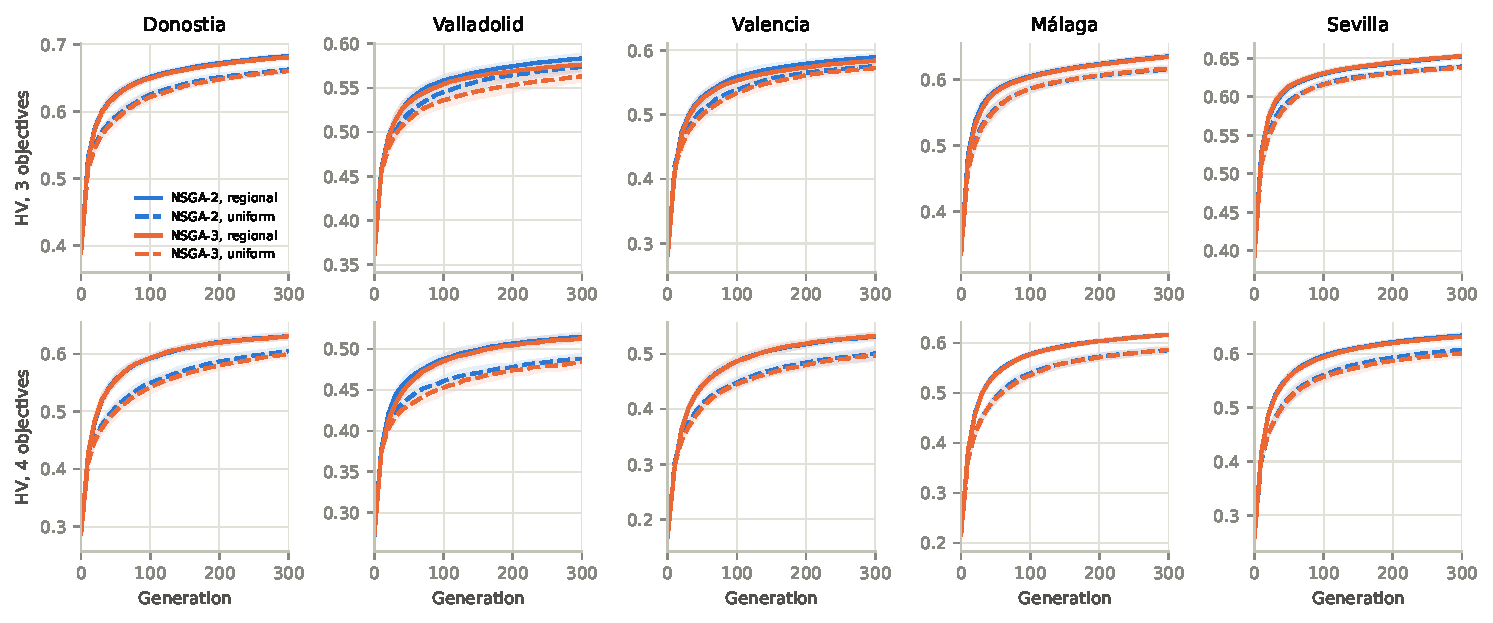
\includegraphics[width=\textwidth]{figures/convergence.pdf}
    \caption{Hypervolume of the front along the generations in the factorial study, in the space of each formulation: mean and standard deviation of 30 runs per variant. Colour: survival strategy; line style: crossover.}
    \label{fig:convergence}
\end{figure}

Table~\ref{tab:hv} and Figure~\ref{fig:convergence} show the factorial study. NSGA-III, designed for problems with many objectives, brings no improvement (last column). With three objectives, the differences are not significant in three cities, and NSGA-II is significantly better in Valladolid ($\hat{A}_{12} = 0.23$ for NSGA-III) and Valencia ($0.29$); with four objectives, no difference is significant ($0.37 \leq \hat{A}_{12} \leq 0.52$). We attribute this to the structure of the problem: the discrete set of sizes already spreads the population along $f_1$, and the guided mutation, rather than the survival step, drives the search (Section~\ref{sec:ablation}). Since NSGA-II is simpler and needs no reference directions, we use it in the rest of the paper and in the service. The two crossovers of this study are compared in Section~\ref{sec:recombination}.

\begin{table}[htbp]
\centering
\small
\caption{The fronts of both formulations (NSGA-II without crossover) scored in both objective spaces: HV3 (containers, unserved people, inequity) and HV4 (plus mean distance), mean (standard deviation) of 30 runs, with the Vargha--Delaney $\hat{A}_{12}$ of the four-objective against the three-objective formulation (Holm-corrected Mann--Whitney U; $^\dagger$: not significant).}
\label{tab:formulation}
\begin{tabular}{lcccccc}
\toprule
& \multicolumn{3}{c}{\textbf{HV3}} & \multicolumn{3}{c}{\textbf{HV4}} \\
\cmidrule(lr){2-4} \cmidrule(lr){5-7}
\textbf{City} & 3 obj. & 4 obj. & $\hat{A}_{12}$ & 3 obj. & 4 obj. & $\hat{A}_{12}$ \\
\midrule
Donostia & 0.7082 (0.0026) & 0.6893 (0.0035) & 0.00 & 0.6194 (0.0101) & 0.6554 (0.0051) & 1.00 \\
Valladolid & 0.6009 (0.0096) & 0.5848 (0.0075) & 0.07 & 0.4766 (0.0194) & 0.5248 (0.0077) & 1.00 \\
Valencia & 0.6143 (0.0060) & 0.6014 (0.0046) & 0.04 & 0.5155 (0.0118) & 0.5480 (0.0078) & 0.99 \\
Málaga & 0.6637 (0.0052) & 0.6420 (0.0034) & 0.00 & 0.5334 (0.0176) & 0.6308 (0.0039) & 1.00 \\
Sevilla & 0.6745 (0.0036) & 0.6581 (0.0025) & 0.00 & 0.5240 (0.0184) & 0.6423 (0.0053) & 1.00 \\
\bottomrule
\end{tabular}
\end{table}


Table~\ref{tab:formulation} scores the fronts of both formulations (NSGA-II without crossover) in both objective spaces. Adding distance as a fourth objective has a small cost in the three-objective space, where the HV3 of the four-objective fronts is between 2.1\% (Valencia) and 3.3\% (Málaga) lower, and a large gain in the four-objective space, where their HV4 is between 5.8\% (Donostia) and 22.6\% (Sevilla) higher. Both differences are significant in every city. The same holds with regional crossover and with NSGA-III.

\begin{figure}[htbp]
    \centering
    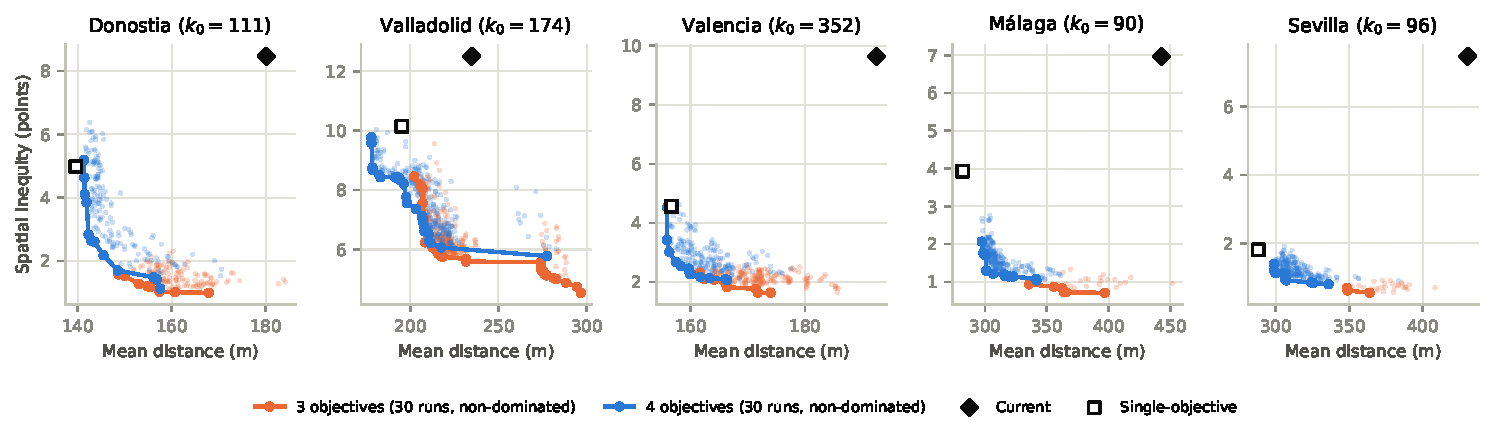
\includegraphics[width=\textwidth]{figures/tradeoff_k0.pdf}
    \caption{Layouts with today's number of containers $k_0$ and no more unserved people than today, from the 30 fronts of each formulation (NSGA-II without crossover), in the plane of mean distance and spatial inequity; lines join the non-dominated ones. Diamond: current layout; square: single-objective algorithm (median of 5 runs).}
    \label{fig:tradeoff}
\end{figure}

Figure~\ref{fig:tradeoff} shows what this means for a planner who keeps today's number of containers. The three-objective fronts concentrate on the fairest layouts and leave accessibility to chance: in Málaga and Sevilla their layouts are 330--400\,m away on average, 50--115\,m more than the single-objective solution. The four-objective fronts cover the whole trade-off, from layouts as accessible as the single-objective solution, and fairer, to layouts nearly as fair as the three-objective ones. In Valladolid and Valencia they include layouts that dominate the single-objective solution in both distance and inequity; in Donostia, Málaga and Sevilla, layouts within 2--15\,m of its distance with less inequity.

\subsection{Recombination}
\label{sec:recombination}
The factorial study shows a large and consistent advantage of the regional crossover over the uniform crossover (Table~\ref{tab:hv}): it wins in all 20 comparisons, with $\hat{A}_{12} \geq 0.87$. This does not mean that recombination helps, only that one crossover is less harmful than the other. To find out, we compared crossovers with no crossover at all, after giving each spatial crossover a fair chance. Both were tuned with the same protocol on two cities (Donostia and Valencia, 10 runs each): the regional crossover over six ranges of region size, from $\rho \in [0.001, 0.005]$ to $[0.1, 0.5]$, and the graph crossover over ten combinations of the number of subgraphs $g \in \{1, 3, 10\}$ and their depth $h \in \{1, \dots, 20\}$. The configuration with the best mean rank over both cities was kept: the smallest regions for the regional crossover ($[0.001, 0.005]$, i.e., 1--16 candidates), and one subgraph of depth 1 (a candidate and its Delaunay neighbours) for the graph crossover. In both cases, the smaller the exchanged region, the better.

\begin{table}[htbp]
\centering
\small
\caption{Recombination (NSGA-II, four objectives): HV4 after 300 generations, mean (standard deviation) of 30 runs, without crossover and with four crossovers: regional and graph crossover with small regions (tuned, Section~\ref{sec:recombination}), regional crossover with large regions (10--50\% of the candidates) and uniform crossover. $\hat{A}_{12}$: probability that a run with the crossover beats a run without it (Holm-corrected Mann--Whitney U; $^\dagger$: not significant).}
\label{tab:recombination}
\resizebox{\textwidth}{!}{%
\begin{tabular}{lccccccccc}
\toprule
& \textbf{None} & \multicolumn{2}{c}{\textbf{Regional, small}} & \multicolumn{2}{c}{\textbf{Graph, small}} & \multicolumn{2}{c}{\textbf{Regional, large}} & \multicolumn{2}{c}{\textbf{Uniform}} \\
\cmidrule(lr){3-4} \cmidrule(lr){5-6} \cmidrule(lr){7-8} \cmidrule(lr){9-10}
\textbf{City} & HV4 & HV4 & $\hat{A}_{12}$ & HV4 & $\hat{A}_{12}$ & HV4 & $\hat{A}_{12}$ & HV4 & $\hat{A}_{12}$ \\
\midrule
Donostia & 0.6554 (0.0051) & 0.6528 (0.0044) & 0.31 & 0.6507 (0.0053) & 0.25 & 0.6302 (0.0063) & 0.00 & 0.6042 (0.0089) & 0.00 \\
Valladolid & 0.5248 (0.0077) & 0.5209 (0.0074) & 0.37$^\dagger$ & 0.5221 (0.0057) & 0.40$^\dagger$ & 0.5147 (0.0049) & 0.13 & 0.4880 (0.0061) & 0.00 \\
Valencia & 0.5480 (0.0078) & 0.5506 (0.0076) & 0.58$^\dagger$ & 0.5490 (0.0104) & 0.54$^\dagger$ & 0.5309 (0.0079) & 0.06 & 0.5005 (0.0131) & 0.00 \\
Málaga & 0.6308 (0.0039) & 0.6316 (0.0047) & 0.58$^\dagger$ & 0.6305 (0.0041) & 0.50$^\dagger$ & 0.6160 (0.0048) & 0.01 & 0.5853 (0.0069) & 0.00 \\
Sevilla & 0.6423 (0.0053) & 0.6446 (0.0053) & 0.63$^\dagger$ & 0.6447 (0.0053) & 0.61$^\dagger$ & 0.6345 (0.0058) & 0.18 & 0.6076 (0.0074) & 0.00 \\
\bottomrule
\end{tabular}}
\end{table}


Table~\ref{tab:recombination} shows the result. Recombination brings no improvement. The tuned crossovers are statistically indistinguishable from no crossover in four cities, and worse in Donostia ($\hat{A}_{12} = 0.31$ and $0.25$); the crossovers with large regions and the uniform crossover are clearly worse in every city ($\hat{A}_{12} \leq 0.18$). Moreover, the best crossovers exchange so few locations that they act as an additional mutation. No crossover is also cheaper: since half of the offspring are unmutated copies of their parents, which need no new evaluation, a run is 1.6 to 2.4 times faster than with the small-region crossovers, and up to three times faster than with the large ones. We therefore recommend, and use in the service, NSGA-II without crossover. In our problem, the locations interact through the Voronoi cells and the shares of their neighbourhoods; exchanging even small, spatially coherent parts between two good layouts breaks those interactions more often than it combines their strengths, while small guided moves improve them.

\subsection{Ablation}
\label{sec:ablation}
\begin{table}[htbp]
\centering
\small
\caption{Ablation of the recommended configuration (NSGA-II, four objectives, no crossover): HV4, mean of 30 runs, with one component removed at a time: the discrete set of sizes (all sizes in the range allowed), the load-guided resizing (random instead), the comparison of $f_2$ in steps (exact values), the local moves of the mutation (all moves to random candidates) and the seeding of the current layout. $\hat{A}_{12}$: probability that a run of the full configuration beats a run without the component (Holm-corrected Mann--Whitney U; $^\dagger$: not significant).}
\label{tab:ablation}
\resizebox{\textwidth}{!}{%
\begin{tabular}{lccccccccccc}
\toprule
& \textbf{Full} & \multicolumn{2}{c}{\textbf{All sizes}} & \multicolumn{2}{c}{\textbf{Random resize}} & \multicolumn{2}{c}{\textbf{Exact $f_2$}} & \multicolumn{2}{c}{\textbf{No local moves}} & \multicolumn{2}{c}{\textbf{No seed}} \\
\textbf{City} & HV4 & HV4 & $\hat{A}_{12}$ & HV4 & $\hat{A}_{12}$ & HV4 & $\hat{A}_{12}$ & HV4 & $\hat{A}_{12}$ & HV4 & $\hat{A}_{12}$ \\
\midrule
Donostia & 0.6554 & 0.5170 & 1.00 & 0.4960 & 1.00 & 0.6465 & 0.84 & 0.6349 & 0.99 & 0.6557 & 0.52$^\dagger$ \\
Valladolid & 0.5248 & 0.3962 & 1.00 & 0.4103 & 1.00 & 0.5183 & 0.72 & 0.5128 & 0.88 & 0.5232 & 0.56$^\dagger$ \\
Valencia & 0.5480 & 0.3011 & 1.00 & 0.3292 & 1.00 & 0.5382 & 0.82 & 0.5251 & 0.96 & 0.5491 & 0.46$^\dagger$ \\
Málaga & 0.6308 & 0.5167 & 1.00 & 0.4955 & 1.00 & 0.6041 & 0.99 & 0.6050 & 1.00 & 0.6292 & 0.61$^\dagger$ \\
Sevilla & 0.6423 & 0.5284 & 1.00 & 0.5262 & 1.00 & 0.6257 & 0.97 & 0.6238 & 1.00 & 0.6458 & 0.31 \\
\bottomrule
\end{tabular}}
\end{table}


Table~\ref{tab:ablation} removes one component of the recommended configuration at a time. The discrete set of sizes and the load-guided resizing are essential: without either of them, the HV4 drops by 18--45\% in every city ($\hat{A}_{12} = 1.00$). Allowing all sizes spreads the population too thinly for layouts of the same size to compete, and random resizing adds and removes containers where they matter least. The local moves of the mutation and the comparison of $f_2$ in steps of 100 people also contribute significantly in every city ($0.72 \leq \hat{A}_{12} \leq 1.00$). Seeding the current layout makes no difference in four cities, and in Sevilla it is slightly worse ($\hat{A}_{12} = 0.31$); its purpose is to guarantee that the front is never worse than the existing deployment, not to speed up the search.

\subsection{The equity measure}
\label{sec:equity_results}
\begin{table}[htbp]
\centering
\small
\caption{Spearman rank correlation between $f_3$ (500\,m blocks, 1\,km neighbourhoods) and other measures, over the layouts with today's number of containers of the 30 fronts of each city (NSGA-II, four objectives, no crossover): $f_3$ with other block sizes and radii, Moran's I of the blocks, and classical non-spatial measures \cite{marsh1994equity}: population-weighted Gini coefficients of the unserved share of each person, of the load of each container and of the distance to the nearest container.}
\label{tab:equity}
\resizebox{\textwidth}{!}{%
\begin{tabular}{lrccccccc}
\toprule
\textbf{City} & \textbf{Layouts} & $f_3$ 250/500 & $f_3$ 1000/2000 & Moran's I & Gini unserved & Gini load & Gini distance & Mean distance \\
\midrule
Donostia & 171 & +0.88 & +0.90 & +0.85 & +0.06 & -0.37 & -0.73 & -0.80 \\
Valladolid & 318 & +0.86 & +0.83 & +0.66 & +0.25 & -0.57 & -0.54 & -0.84 \\
Valencia & 192 & +0.65 & +0.86 & +0.75 & -0.31 & -0.41 & -0.20 & -0.62 \\
Málaga & 237 & +0.80 & +0.90 & +0.75 & +0.29 & +0.27 & -0.51 & -0.81 \\
Sevilla & 212 & +0.72 & +0.83 & +0.68 & +0.21 & +0.21 & -0.41 & -0.65 \\
\bottomrule
\end{tabular}}
\end{table}


Table~\ref{tab:equity} correlates $f_3$ with other measures over the layouts with today's number of containers of the 30 fronts of each city. $f_3$ is robust to its parameters: with blocks of 250\,m and neighbourhoods of 500\,m, or with blocks of 1\,km and neighbourhoods of 2\,km, it ranks the layouts in a similar order (Spearman $\rho$ between 0.65 and 0.90). The comparison of crossovers does not depend on these parameters either (Table~\ref{tab:sensitivity}): the regional crossover beats the uniform crossover in every city with both alternative settings ($\hat{A}_{12} \geq 0.96$). Moran's I of the blocks, computed on the same fixed support, is also correlated with $f_3$ ($0.66 \leq \rho \leq 0.85$): the intuition of the earlier formulation was sound, its shortcomings were the changing support and the insensitivity to magnitude. Conversely, the classical non-spatial measures rank the layouts differently: the Gini coefficient of the unserved share of each person is almost unrelated to $f_3$ ($-0.31 \leq \rho \leq 0.29$), and the Gini coefficient of the loads is weakly and inconsistently related to it ($-0.57 \leq \rho \leq 0.27$). They measure how unequal the shortage is, not where it is. Finally, $f_3$ is negatively correlated with the mean distance ($-0.62 \leq \rho \leq -0.84$) and with the Gini coefficient of distances: fairer layouts spread containers towards less dense areas, which lengthens the average walk, the trade-off that motivates $f_4$.

\begin{table}[htbp]
\centering
\small
\caption{Sensitivity of the comparison between regional (large regions) and uniform crossover to the parameters of $f_3$ (NSGA-II, four objectives, 30 runs): HV4 with blocks of 250\,m and neighbourhoods of 500\,m, and with blocks of 1\,km and neighbourhoods of 2\,km (each normalized among its own runs), and $\hat{A}_{12}$ of regional against uniform (all differences significant, $p < 10^{-9}$).}
\label{tab:sensitivity}
\begin{tabular}{lcccccc}
\toprule
& \multicolumn{3}{c}{\textbf{250\,m / 500\,m}} & \multicolumn{3}{c}{\textbf{1\,km / 2\,km}} \\
\cmidrule(lr){2-4} \cmidrule(lr){5-7}
\textbf{City} & Regional & Uniform & $\hat{A}_{12}$ & Regional & Uniform & $\hat{A}_{12}$ \\
\midrule
Donostia & 0.5371 & 0.5020 & 0.99 & 0.7169 & 0.6912 & 1.00 \\
Valladolid & 0.4522 & 0.4339 & 0.96 & 0.5479 & 0.5211 & 1.00 \\
Valencia & 0.4522 & 0.4261 & 0.99 & 0.6050 & 0.5787 & 0.98 \\
Málaga & 0.5192 & 0.4800 & 1.00 & 0.6053 & 0.5691 & 1.00 \\
Sevilla & 0.4857 & 0.4452 & 1.00 & 0.5983 & 0.5615 & 1.00 \\
\bottomrule
\end{tabular}
\end{table}


\subsection{How accessible are the solutions?}
\begin{table}[htbp]
\centering
\small
\caption{Mean distance (m) with today's number of containers $k_0$: Lagrangian lower bound of the $p$-median problem \cite{beasley1993lagrangean}, best known solution (Lagrangian heuristic or alternating local search), single-objective genetic algorithm (median of 5 runs) and the most accessible layout of the four-objective fronts no worse than the current layout in unserved people and inequity (median of 30 runs); in brackets, the gap to the best known solution. The last column is the inequity of the best known solution.}
\label{tab:bounds}
\begin{tabular}{lrrrrrr}
\toprule
\textbf{City} & $k_0$ & \textbf{Lower bound} & \textbf{Best known} & \textbf{Single-obj.} & \textbf{Front} & \textbf{Ineq. best known (pts)} \\
\midrule
Donostia & 111 & 130.5 & 132.2 & 139.6 (+5.6\%) & 143.4 (+8.4\%) & 8.8 \\
Valladolid & 174 & 161.5 & 168.5 & 195.2 (+15.8\%) & 181.1 (+7.5\%) & 12.2 \\
Valencia & 352 & 140.3 & 148.4 & 156.7 (+5.6\%) & 158.4 (+6.7\%) & 4.3 \\
Málaga & 90 & 269.8 & 279.6 & 281.9 (+0.8\%) & 302.5 (+8.2\%) & 4.6 \\
Sevilla & 96 & 277.6 & 288.2 & 288.2 (+0.0\%) & 305.4 (+6.0\%) & 2.7 \\
\bottomrule
\end{tabular}
\end{table}


With today's number of containers, minimizing $f_4$ alone is the $p$-median problem. Its Lagrangian relaxation gives a lower bound on the mean distance that any layout can achieve \cite{beasley1993lagrangean}, and its subproblems, improved by an alternating local search, give good feasible layouts. Table~\ref{tab:bounds} shows that the best known solutions are within 1.3--5.8\% of the lower bound, so the accessibility optimum is tightly bracketed. The most accessible layout of the four-objective fronts that is no worse than today's in unserved people and inequity is 6.0--8.4\% farther than the best known solution, a moderate price for being fair and serving at least as many people; and those best known solutions are themselves unfair (up to 12.2 inequity points in Valladolid). The single-objective algorithm of the service is close to the best known solution in Málaga and Sevilla, but 15.8\% above it in Valladolid, which shows room for improvement in that algorithm too.

\subsection{Comparison with the current layouts}
\begin{table}[htbp]
\centering
\small
\caption{Layouts with today's number of containers $k_0$: the current one; the single-objective genetic algorithm (median of 5 runs); and, among the layouts of each front that are no worse than the current one in unserved people and inequity, the fairest and the one with the shortest mean distance (medians over 30 runs, NSGA-II without crossover). Distances are straight-line and population-weighted.}
\label{tab:k0}
\begin{tabular}{llrrrr}
\toprule
\textbf{City} & \textbf{Layout} & \textbf{Unserved} & \textbf{Inequity (pts)} & \textbf{Mean dist. (m)} & \textbf{95\% within (m)} \\
\midrule
\multirow{5}{*}{\shortstack[l]{Donostia\\($k_0=111$)}} & Current & 78,063 & 8.5 & 180 & 435 \\
 & Single-objective GA & 68,991 & 5.0 & 140 & 285 \\
 & 3 obj., fairest & 69,955 & 1.2 & 161 & 359 \\
 & 4 obj., fairest & 71,360 & 1.9 & 156 & 334 \\
 & 4 obj., shortest distance & 69,101 & 4.6 & 143 & 300 \\
\midrule
\multirow{5}{*}{\shortstack[l]{Valladolid\\($k_0=174$)}} & Current & 111,812 & 12.5 & 235 & 650 \\
 & Single-objective GA & 99,484 & 10.1 & 195 & 415 \\
 & 3 obj., fairest & 110,432 & 5.9 & 225 & 523 \\
 & 4 obj., fairest & 109,851 & 6.4 & 221 & 496 \\
 & 4 obj., shortest distance & 99,936 & 9.1 & 181 & 425 \\
\midrule
\multirow{5}{*}{\shortstack[l]{Valencia\\($k_0=352$)}} & Current & 455,407 & 9.6 & 193 & 517 \\
 & Single-objective GA & 444,497 & 4.6 & 157 & 326 \\
 & 3 obj., fairest & 447,145 & 2.0 & 172 & 378 \\
 & 4 obj., fairest & 446,503 & 2.4 & 166 & 357 \\
 & 4 obj., shortest distance & 444,497 & 3.4 & 158 & 338 \\
\midrule
\multirow{5}{*}{\shortstack[l]{Málaga\\($k_0=90$)}} & Current & 438,324 & 7.0 & 443 & 1525 \\
 & Single-objective GA & 438,324 & 3.9 & 282 & 558 \\
 & 3 obj., fairest & 438,324 & 1.0 & 379 & 906 \\
 & 4 obj., fairest & 438,324 & 1.3 & 319 & 711 \\
 & 4 obj., shortest distance & 438,324 & 2.0 & 303 & 663 \\
\midrule
\multirow{5}{*}{\shortstack[l]{Sevilla\\($k_0=96$)}} & Current & 592,162 & 7.5 & 431 & 896 \\
 & Single-objective GA & 591,205 & 1.8 & 288 & 573 \\
 & 3 obj., fairest & 591,205 & 0.7 & 374 & 843 \\
 & 4 obj., fairest & 591,205 & 1.0 & 327 & 691 \\
 & 4 obj., shortest distance & 591,205 & 1.5 & 305 & 631 \\
\bottomrule
\end{tabular}
\end{table}


In all 30 runs of every city, the four-objective front contained a layout with $k_0$ containers that is better than the current one in unserved people, inequity and mean distance at once. Table~\ref{tab:k0} details the typical (median) layouts. Relocating the existing containers reduces both the shortage and its inequity: in Donostia, the unserved population falls by 9\% (from 78,063 to about 71,400), the inequity from 8.5 to 1.9 points and the mean distance from 180 to 156\,m; in Valencia, the inequity falls from 9.6 to 2.4 points and the distance from 193 to 166\,m. In Málaga and Sevilla, where the shortage is fixed by the number of containers, relocation cannot serve more people, but it divides the inequity by 5.4 and 7.5, respectively, and shortens the mean distance by more than 100\,m. Figure~\ref{fig:map} shows where this happens in Donostia: in the current layout, the shortage is concentrated in the central and southern districts, which have up to 25 points more unserved people than the city average, while the north-east has spare capacity; in the front layout, the differences between neighbourhoods shrink to a few points in most of the city.

As noted in Section~\ref{problem_definition}, $f_2$ is close to its lower bound $P - \alpha|S|$ for almost every layout of the fronts, as no city has enough containers for its population. The trade-off between more containers and fewer unserved people is therefore nearly arithmetic, and the value of the optimization lies in where the containers go: the equity and accessibility of the layouts of each size.

\begin{figure}[htbp]
    \centering
    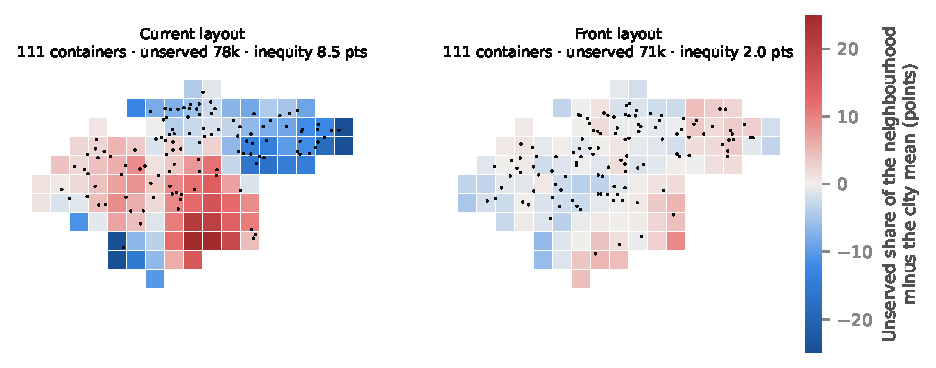
\includegraphics[width=0.95\textwidth]{figures/map_donostia.pdf}
    \caption{Donostia, 500\,m blocks colored by the unserved share of their 1\,km neighbourhood minus the city average, for the current layout (left) and the fairest layout with the same number of containers and no more unserved people, from the four-objective run with the median such fairness (right). Dots are the containers.}
    \label{fig:map}
\end{figure}

\subsection{Integration in a data space}
The method is deployed as a service of the CitCom.ai data space, which reads the inventory of containers of a city through NGSI-LD (Smart Data Models \texttt{WasteContainer} entities) from the city's connector, and the population from GHS-POP, so it can be applied to any city that publishes its containers. A job runs in a single low-priority process. With the recommended configuration (NSGA-II, four objectives, no crossover, 300 generations, 100 individuals), it computes the front of Valencia in under a minute on one core of the cluster, and in a few minutes in the deployed service, where it runs at low priority on a shared node with the 8,308 candidate sites of the city's data. The planner can then browse the front and display any of its layouts on a map, compared with the current one.

\section{Conclusions}
\label{conclusions}
Cities, with their high population density, account for most of the oil and other fats consumed for culinary purposes, whether for domestic use or services. In the current context of the fight against climate change and the achievement of the SDGs, cities play a critical role, as they are responsible for the proper treatment of waste and for trying to implement the necessary measures to combat global warming. In this sense, UCO can be a valuable ally, given its ease of reuse as biodiesel, which produces clean and sustainable energy. However, planning urban infrastructure for its collection using containers equipped for this purpose is not always easy. These types of facilities have often grown organically alongside cities, resulting in deficient access in terms of coverage and equity, which discourages greater collection.

In this paper, we introduced a multi-objective facility location formulation and a tailored evolutionary algorithm for the placement of UCO collection containers. The model integrates four planning criteria: the number of containers, the population left without capacity in Voronoi-based service areas, the spatial equity of that shortage, and the distance to the nearest container. We showed that Moran's index, a natural candidate for the equity criterion, is ill-posed as an objective: it is fixed by the number of observations in small solutions, nearly constant in realistic ones, and blind to the magnitude of the shortage. We replaced it with a measure on a fixed spatial support, the population-weighted dispersion of the unserved share between neighbourhoods, which is comparable across solutions of any size and grows only when the shortage is both unequal and spatially concentrated. We showed that this measure is robust to its parameters and ranks solutions differently from the classical non-spatial equity measures. Methodologically, we adapted NSGA-II to sets of locations with a discrete set of network sizes and three problem-specific operators: a partition crossover between parents of the same size with load-guided repair, a mutation that moves containers towards the people they serve, and an initialization with equal-population cells. An extensive study on real data from five Spanish cities showed that the size management and the load-guided resizing are essential to the quality of the fronts; that NSGA-III brings no improvement over NSGA-II, even with four objectives; that, in the same computing time, the proposed configuration improves the hypervolume of a mutation-driven one by 4--10\% and that of seven crossovers of the literature, in their original form, by 3--11\%; that same-size mating and load-guided repair are what make recombination work, for our crossover and for the others, so that crossovers that exchange large regions reach the level of ours once they have them; that the exact decomposition of two layouts into independent components, on which partition crossover rests in other problems, leaves one component with most of the differences, and imposing tiles works better; that the equal-population seeds alone are fairer and more accessible than today's layouts; and that adding distance as an objective costs little in the other objectives while covering the trade-off between equity and accessibility that the three-objective formulation leaves to chance. The most accessible fair layouts are within 6--9\% of the best known solutions of the corresponding $p$-median problem, whose optimum we bracketed within 6\% with a Lagrangian bound.

From an applied perspective, the fronts are directly usable by planners. With today's number of containers, every front contained layouts that are better than the current deployment in unserved population, spatial inequity (by a factor of 2 to 7) and mean distance at once, and layouts nearly as accessible as those of a single-objective optimizer but fairer. The fronts also make explicit what each additional container buys, and show that in cities with a strong shortage of capacity, such as Málaga and Sevilla, relocation alone cannot serve more people, but it can make the shortage fair.

We recognize the limitations that shape future research. First, no real cost data were available, so the size of the network stands for its cost; per-site installation and maintenance costs can replace it directly. Second, with four objectives most of the population is non-dominated, which weakens the pressure towards the extremes of the front: the fairest layouts are somewhat less fair than with three objectives. Larger populations, or archives per network size, could recover them at a higher computational cost. The proposed configuration improves most of the front but not its fairest end, which needs more generations or the comparison of inequity in each tile; an operator that handles the non-additive objective directly is an open question. Once mating and repair are in place, the differences between the best crossovers are within 1\%, so the remaining room lies less in the shape of the exchanged regions than in the mutation, the initialization and the treatment of inequity; partitions that follow the structure of the city, such as districts or the street network, are still worth testing. Third, distances are straight-line; walking distances on the street network would be more realistic. Fourth, the model assumes static demand and that citizens use the nearest container; data on container filling and on actual use would make it more realistic. Finally, combining location with collection routing would capture the operational cost of the network.

Taken together, our findings show that integrating spatial equity into multi-objective evolutionary optimization provides a flexible framework for siting urban waste collection infrastructure, provided the equity measure is well-posed for optimization. The methodological lessons presented here, equity measured on a fixed spatial support, problem-specific mutation and size management, and recombination that uses the locality of the objectives rather than blind recombination, and bounds on the classical single-objective problem to assess solution quality, carry over to other urban services that face similar trade-offs between cost, coverage and fairness. The method is deployed as an open-source service of a data space, so municipalities that publish their container inventories can use it directly.

%\backmatter

% \bmsection*{Author contributions}
% This is an author contribution text. This is an author contribution text. This is an author contribution text. This is an author contribution text. This is an author contribution text.

\bmsection*{Acknowledgments}
This work is partially funded by the Spanish Ministry of Science and Innovation under the project PID2021-123673OB-C31, project TED2021-131295B-C32 from the State Research Agency, and DIGITAL2022 CLOUDAI02/S8760000 from the European Commission. 

% \bmsection*{Financial disclosure}

% None reported.

\bmsection*{Conflict of interest}

The authors declare no potential conflict of interests.

\bibliography{references}

\end{document}
    